\chapter{Dexterous Fine-Tuning for Hand Policies}
\label{cha:deft}

\section{Introduction}
\label{sec:intro}

\begin{figure}[H]
\centering
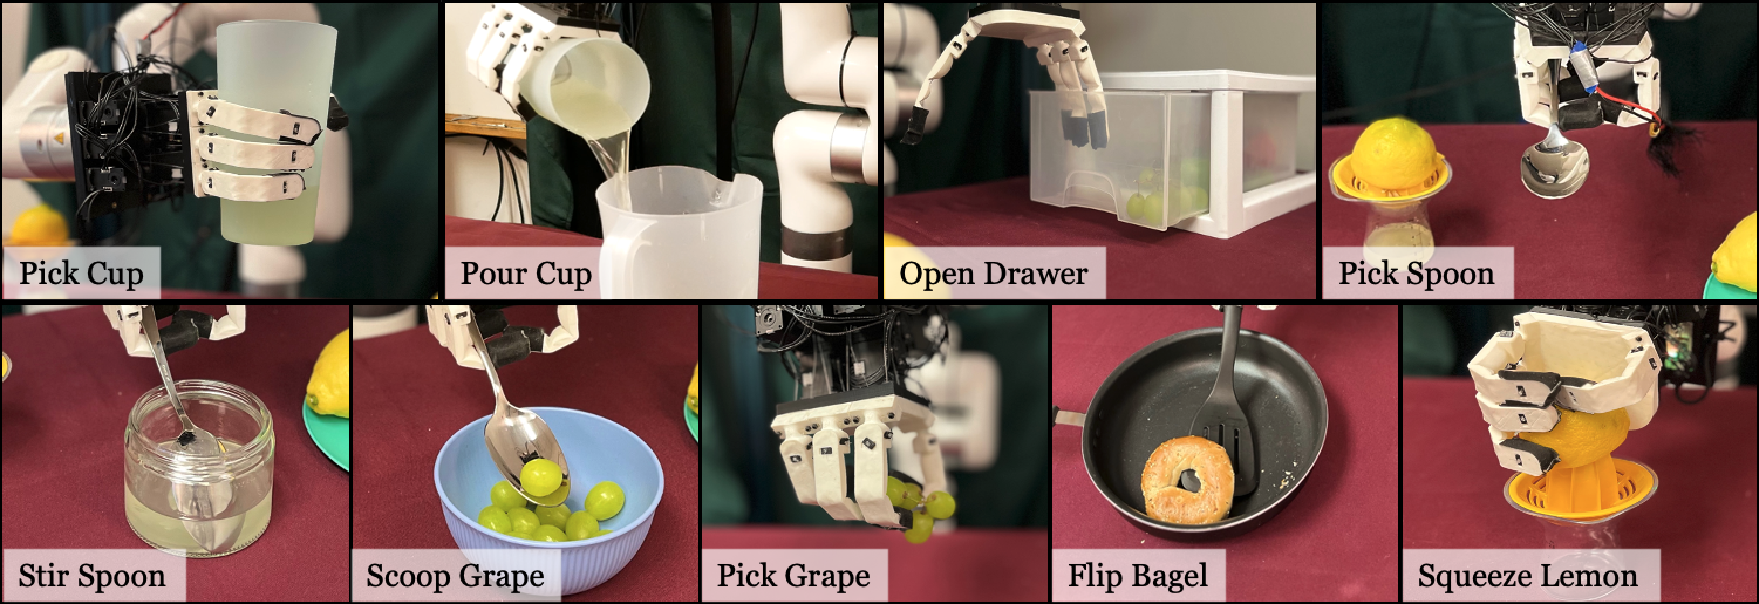
\includegraphics[width=\linewidth]{figs/teaser.pdf}
\vspace{-0.2in}
  \caption{\small We present \ours, a novel approach that can learn complex, dexterous tasks in the real world in an efficient manner. \ours manipulates tools and soft objects without any robot demonstrations.}
 \label{fig:teaser}
\end{figure}


The longstanding goal of robot learning is to build robust agents that can perform long-horizon tasks autonomously. This could for example mean a self-improving robot that can build furniture or an agent that can cook for us. A key aspect of most tasks that humans would like to perform is that they require complex motions that are often only achievable by hands--consider the task of tying shoelaces. Such a task would be impossible with a parallel jaw gripper. Therefore, in this work, we investigate real-world dexterous manipulation, its challenges, and its deployment in the real world. 

A key challenge in deploying  policies in the real world, especially with robotic hands, is that there exist many failure modes. Controlling a dexterous hand is much harder than end-effectors due to larger action spaces and complex dynamics. This problem becomes even more difficult when contacts with objects are more involved, as there can be many points of contact on a robotic hand. To address this, one option is to \textit{improve} directly in the real world via \textit{practice}. Traditionally, reinforcement learning (RL) and imitation learning (IL) techniques have been used to deploy hands-on tasks such as in-hand rotation or grasping. To be proficient at any skill a lot of practice or data is needed. This is often the case as setups are built so that it is either easy to simulate in the real world or robust to practice. However, the real world contains tasks that one cannot simulate (such as manipulation of soft objects like food) or difficult settings in which the robot cannot practice (sparse long-horizon tasks like assembly). How can we build an approach that can scale to such tasks? 

There are several issues with current approaches for practice and improvement in the real world. Robot hardware often breaks, especially with the amount of contact to learn dexterous tasks like operating tools. We thus investigate using a \textit{soft anthropomorphic hand} ~\cite{mannam2023framework}, which can easily run in the real world without failures or breaking. This soft anthropomorphic hand is well-suited to our approach as it is flexible and can gently handle object interactions. The hand does not get damaged by the environment and is robust to continuous data collection. Due to its human-like proportions and morphology, retargeting human hand grasps to robot hand grasps is made simpler.  

Unfortunately, this hand is difficult to simulate due to its softness. Directly learning from scratch is also difficult as we would like to build \textit{generalizable policies}, and not practice for every new setting.  To achieve efficient real-world learning, we must learn a prior for reasonable behavior to explore using useful actions.  Many previous methods rely on in-domain human demonstrations that are manually collected by a human operator or demonstrator \cite{shaw2022video, zhao2023learning, pomerleau1988alvinn, mandlekar2021matters}. Due to recent advances in large-scale computer vision, we propose \textit{leveraging human data to learn priors} for dexterous tasks, and improving on such priors in the real world. We aim to use the vast corpus of internet data to define this prior. What is the best way to combine human priors with online practice, especially for hand-based tasks? When manipulating an object, the first thing one thinks about is where on the object to make contact, and how to make this contact. Then, we think about how to move our hands \textit{after the contact}. In fact, this type of prior has been studied in computer vision and robotics literature as \textit{visual affordances} \cite{fouhey2015defense, bahl2023affordances, hap, hotspots, 100doh, hoi, hoi4d, wang2017binge}. In our approach, \ours, we build dexterous grasp affordances which predict the contact point, hand pose at contact, and post-contact trajectory. To improve upon these, we introduce a sampling-based approach similar to the Cross-Entropy Method (CEM) to fine-tune. Specifically, we tune the robot hand grasp, the pose, and the post-grasp trajectory all in the real world for a variety of tasks.  This method enables iterative real-world improvement in less than an hour. 

In summary, our approach (\ours) executes real-world learning on a soft robot hand with only a few trials in the real world.  To facilitate this efficiently, we train priors on human motion from internet videos. We introduce 9 challenging tasks (as seen in Figure \ref{fig:teaser}) that are difficult even for trained operators to perform: Picking a Cup, Pouring Lemonade, Opening a Drawer, Picking a Spoon, Scooping a Grape, Stirring a Spoon, Picking Grapes, Flipping a Bagel, and Squeezing a Lemon.  While our method begins to show good success on these tasks with real-world fine-tuning, more investigation is required to complete these tasks more effectively. Please see our website for details and videos at \url{http://dexterousfinetuning.github.io}.
